\documentclass{ijcaArticle}
\setcounter{page}{1}
\ijcaVolume{*}
\ijcaNumber{*}
\ijcaYear{2024}
\ijcaMonth{--------}

\usepackage{amsmath,amssymb,amsfonts}
\usepackage{textcomp}
\usepackage{xcolor}
\usepackage{grffile}
\usepackage{graphicx}
\graphicspath{{figures/}{./}{Thesis/}}

\hyphenpenalty=5000
\exhyphenpenalty=5000
\sloppy

\begin{document}

\title{Comparative Performance and Computational Complexity Analysis of Pre-Trained Deep Learning Models for Citrus Fruit Disease Classification}

\author{ 
   \large Nur E Jannatul Farjana \\[-3pt]
   \normalsize Dept. of Computer Science and Engineering \\[-3pt]
   \normalsize International University of Business Agriculture and Technology \\[-3pt]
   \normalsize Uttara, Dhaka-1230, Bangladesh \\[-3pt]
  \and
   \large Abdullah Miraz \\[-3pt]
   \normalsize Dept. of Computer Science and Engineering \\[-3pt]
   \normalsize International University of Business Agriculture and Technology \\[-3pt]
   \normalsize Uttara, Dhaka-1230, Bangladesh \\[-3pt]
  \and
   \large Krishna Das \\[-3pt]
   \normalsize Dept. of Computer Science and Engineering \\[-3pt]
   \normalsize International University of Business Agriculture and Technology \\[-3pt]
   \normalsize Uttara, Dhaka-1230, Bangladesh \\[-3pt]
}

\terms{Algorithms, Experimentation, Performance}
\keywords{Transfer Learning, Convolutional Neural Networks, Citrus Disease Classification, Performance Metrics, Computational Complexity, MobileNetV2}

\maketitle

\begin{abstract} 
Citrus fruit diseases represent a critical threat to global agricultural productivity, causing severe financial and crop yield losses when left undetected or untreated. This study presents a systematic comparative evaluation of transfer learning and deep convolutional neural network (CNN) architectures to classify citrus fruit diseases efficiently and accurately. Using an experimental dataset comprising 1,463 high-resolution images categorized across four distinct classes---canker, black spot, greening, and healthy---four prominent pre-trained architectures (MobileNetV2, InceptionV3, ResNet50, and VGG19) are fine-tuned and benchmarked. The evaluation encompasses both diagnostic performance (accuracy, precision, recall, and F1-score) and computational complexity (training time, inference latency, and memory utilization). Experimental results demonstrate that MobileNetV2 achieves superior diagnostic accuracy of 96.77\% with minimal memory consumption (9.82~MB) and fast inference (83.67~s for the test partition), whereas ResNet50 demonstrates suboptimal generalization on the target dataset with an accuracy of 58.21\%. The findings highlight the critical importance of architectural selection and demonstrate the practical viability of lightweight transfer learning models for automated, edge-deployable citrus disease diagnosis systems.
\end{abstract}

\section{Introduction}

Agriculture is a cornerstone of the national economy in Bangladesh, where sustained productivity directly underpins food security and economic resilience. Modern agricultural initiatives aim to maximize food production and quality while minimizing operational overhead \cite{p1,p2,p19}. Driven by population growth and climatic variability, the agricultural sector is progressively adopting precision agriculture (PA) technologies to optimize crop management \cite{p10,p21}. Precision agriculture incorporates intelligent computational methods for pest localization, weed detection, yield estimation, and automated disease diagnosis \cite{p3}.

Citrus cultivation in Bangladesh has grown substantially, with total production expanding from 19,163 tonnes in 1973 to 175,325 tonnes in 2022, representing an average annual growth rate of 5.61\% \cite{p22}. Field surveys conducted across citrus plantations in the Sylhet region identified canker, scab, dieback, and greening (Huanglongbing) as the primary pathological threats affecting multiple commercial citrus species \cite{p5,p19}. Early detection of these pathological conditions is imperative to prevent disease proliferation and mitigate financial loss. Convolutional Neural Networks (CNNs) have emerged as the state-of-the-art methodology for visual disease diagnosis across various botanical domains \cite{p5}. Canonical architectures such as AlexNet, VGG16, VGG19, InceptionV3, ResNet, and DenseNet have established high efficacy in plant leaf and fruit disease recognition.

\subsection{Context and Background}

In developing nations, agricultural plant diseases impose substantial burdens on rural livelihoods and regional food supplies \cite{p6,p8}. Crop cultivation represents the primary source of income and staple food production across Bangladesh. However, seasonal disease outbreaks frequently diminish harvest yields, rendering disease control a key governmental and scientific priority \cite{p6}. High-resolution digital imaging integrated with machine learning and deep learning frameworks enables automated, non-invasive pathology analysis \cite{p19,p20}. Early automated localization of lesion sites through computer vision significantly enhances targeted intervention efficacy. Agricultural surveys report that over 39,678 acres are dedicated to intensive fruit and crop farming in Bangladesh, highlighting the scale at which automated diagnostic tools are required \cite{p7,p6}.

\subsection{Research Motivation}

Numerous prior studies have investigated supervised deep learning models for citrus disease classification \cite{p2, p5, p8}. Although deep models such as AlexNet and VGG19 achieve competitive classification rates, they typically incur substantial parameter footprints, extensive GPU memory demands, and protracted training durations \cite{p5}. Furthermore, most existing studies focus solely on classification accuracy without conducting rigorous computational complexity or hardware feasibility assessments. To address this research gap, this study conducts an empirical investigation evaluating both classification efficacy and computational overhead across prominent deep transfer learning models.

\subsection{Objectives and Scope}
The primary objectives of this study are:
\begin{itemize}
    \item To implement and fine-tune four prominent pre-trained CNN architectures (MobileNetV2, InceptionV3, ResNet50, and VGG19) for multi-class citrus fruit disease classification.
    \item To perform a rigorous dual-faceted evaluation analyzing both predictive performance metrics (precision, recall, F1-score, accuracy) and computational complexity parameters (training duration, inference latency, parameter footprint, memory consumption).
    \item To identify the most practical, resource-efficient architecture suitable for deployment in resource-constrained edge devices and field agricultural monitoring systems.
\end{itemize}

\subsection{Significance of Research}
This research contributes an empirical benchmark of transfer learning architectures for citrus pathology, establishing quantitative trade-offs between classification accuracy and computational resource requirements. The findings provide clear engineering guidelines for deploying deep learning models in automated agricultural decision-support systems.

The remainder of this paper is organized as follows: Section~\ref{sec:literature_review} presents a review of related literature. Section~\ref{sec:proposed_methodology} details the proposed methodology, dataset preparation, and transfer learning framework. Section~\ref{sec:result_and_discussion} provides the experimental results, performance analysis, and complexity comparisons. Finally, Section~\ref{sec:conclusion} concludes the paper with discussions on limitations and future research directions.

\section{Literature Review}
\label{sec:literature_review}

The agricultural sector sustains approximately 87\% of the rural population in Bangladesh through direct or indirect employment \cite{p9}. Consequently, early automated plant pathology diagnosis using computer vision has attracted substantial research interest. This section summarizes recent advancements in plant disease detection.

Ahmed and Muqit \cite{p2} developed a deep neural network model for automated citrus fruit and leaf disease detection. Their three-stage workflow comprised data acquisition, image pre-processing, and CNN classification. Evaluating 2,293 images from PlantVillage across multiple citrus classes yielded an accuracy of 94.55\%, though the per-class sample size remained limited.

Balafas et al. \cite{p3} conducted a comparative analysis evaluating classical machine learning classifiers (SVM, Random Forest, SGD) against deep learning models (InceptionV3, VGG16, VGG19) on citrus leaf images, demonstrating the superior representational capacity of deep CNN architectures in complex field imagery.

\begin{table*}[t]
\tabcolsep4pt
\tbl{Comprehensive Summary of Related Literature on Citrus and Plant Disease Detection}{
\begin{tabular}{|c|l|c|p{4.2cm}|p{2.8cm}|p{3.8cm}|c|}
\hline
\textbf{No.} & \textbf{Author} & \textbf{Year} &
\textbf{Class Types} & \textbf{Dataset Size} & \textbf{Classifier Architecture} &
\textbf{Accuracy} \\
\hline
1 & R. Sujatha et al. \cite{p10} & 2021 &
Black spot, Canker, Greening, Melanose, Healthy &
609 images &
LSVM, SGD, RF, InceptionV3, VGG16, VGG19 &
89.5\% \\
\hline
2 & Khattak et al. \cite{p7} & 2021 &
Black spot, Canker, Scab, Greening, Melanose, Healthy &
2293 (Fruits+Leaves) &
Custom CNN + Softmax &
94.55\% \\
\hline
3 & A. Elaraby et al. \cite{p5} & 2022 &
Anthracnose, Black spot, Canker, Scab, Greening, Melanose &
759 (Fruits+Leaves) &
AlexNet, VGG19 &
94.0\% \\
\hline
4 & S. Parez et al. \cite{p18} & 2023 &
Multiple plant pathological conditions &
Plant leaves &
Lightweight CNN + Softmax &
99.0\% \\
\hline
5 & Dehuan Luo et al. \cite{p11} & 2023 &
Anthracnose, Canker, Melanosis, Scab, Brown Spot, Leaf Miner &
3202 images &
Light-SA YOLOv8 &
92.6\% \\
\hline
6 & Madhusudan G. et al. \cite{p17} & 2023 &
Black spot, Melanose, Canker, Greening, Healthy &
609 RGB images &
CNN, ResNet152V2, DenseNet121, InceptionResNetV2 &
98.0\% \\
\hline
7 & Poonam Dhiman et al. \cite{p12} & 2023 &
HLB, Black spot, Melanose, Canker, Scab &
2950 images &
CNN + LSTM &
98.25\% \\
\hline
8 & W. G{\'o}mez-Flores et al. \cite{p13} & 2024 &
HLB, Greasy spot, Deficiencies, Citrus Mite, Red scale &
953 images &
DNN, Transfer Learning &
-- \\
\hline
9 & Nouman Butt et al. \cite{p14} & 2024 &
Canker, Citrus scab, Black spot &
2184 images &
SVM, KNN &
99.6\% \\
\hline
10 & J. Shermila et al. \cite{p15} & 2024 &
Fruit blight, Greening, Scab, Melanoses &
759 images &
Custom CNN + LSTM &
96.0\% \\
\hline
11 & A.K. Saini et al. \cite{p16} & 2024 &
Anthracnose, Melanose, Brown Spot &
759 images &
SADCNN-ORBM &
99.76\% \\
\hline
\end{tabular}}
\label{tab:citrus_comparison}
\end{table*}

Elaraby et al. \cite{p5} explored deep learning optimization strategies for classifying black spot, canker, greening, and melanose using AlexNet and VGG19, reporting 94\% accuracy on a multi-class dataset. Sujatha et al. \cite{p10} proposed a mobile-assisted plant leaf disease diagnostic framework leveraging deep models for field deployment. Hasan et al. \cite{p6,p24} utilized transfer learning with deep neural networks for identifying diseases in regional Bangladeshi crops, demonstrating that pre-trained weights significantly accelerate convergence on limited datasets. Table~\ref{tab:citrus_comparison} provides a structured summary of related literature on citrus and crop disease detection.

\section{Proposed Methodology}
\label{sec:proposed_methodology}

The overall experimental workflow comprises dataset acquisition, structured data partitioning, image augmentation, transfer learning model construction, hyperparameter optimization, and comprehensive evaluation. The end-to-end framework is depicted in Figure~\ref{fig:research design}.

\begin{figure}[t]
    \centerline{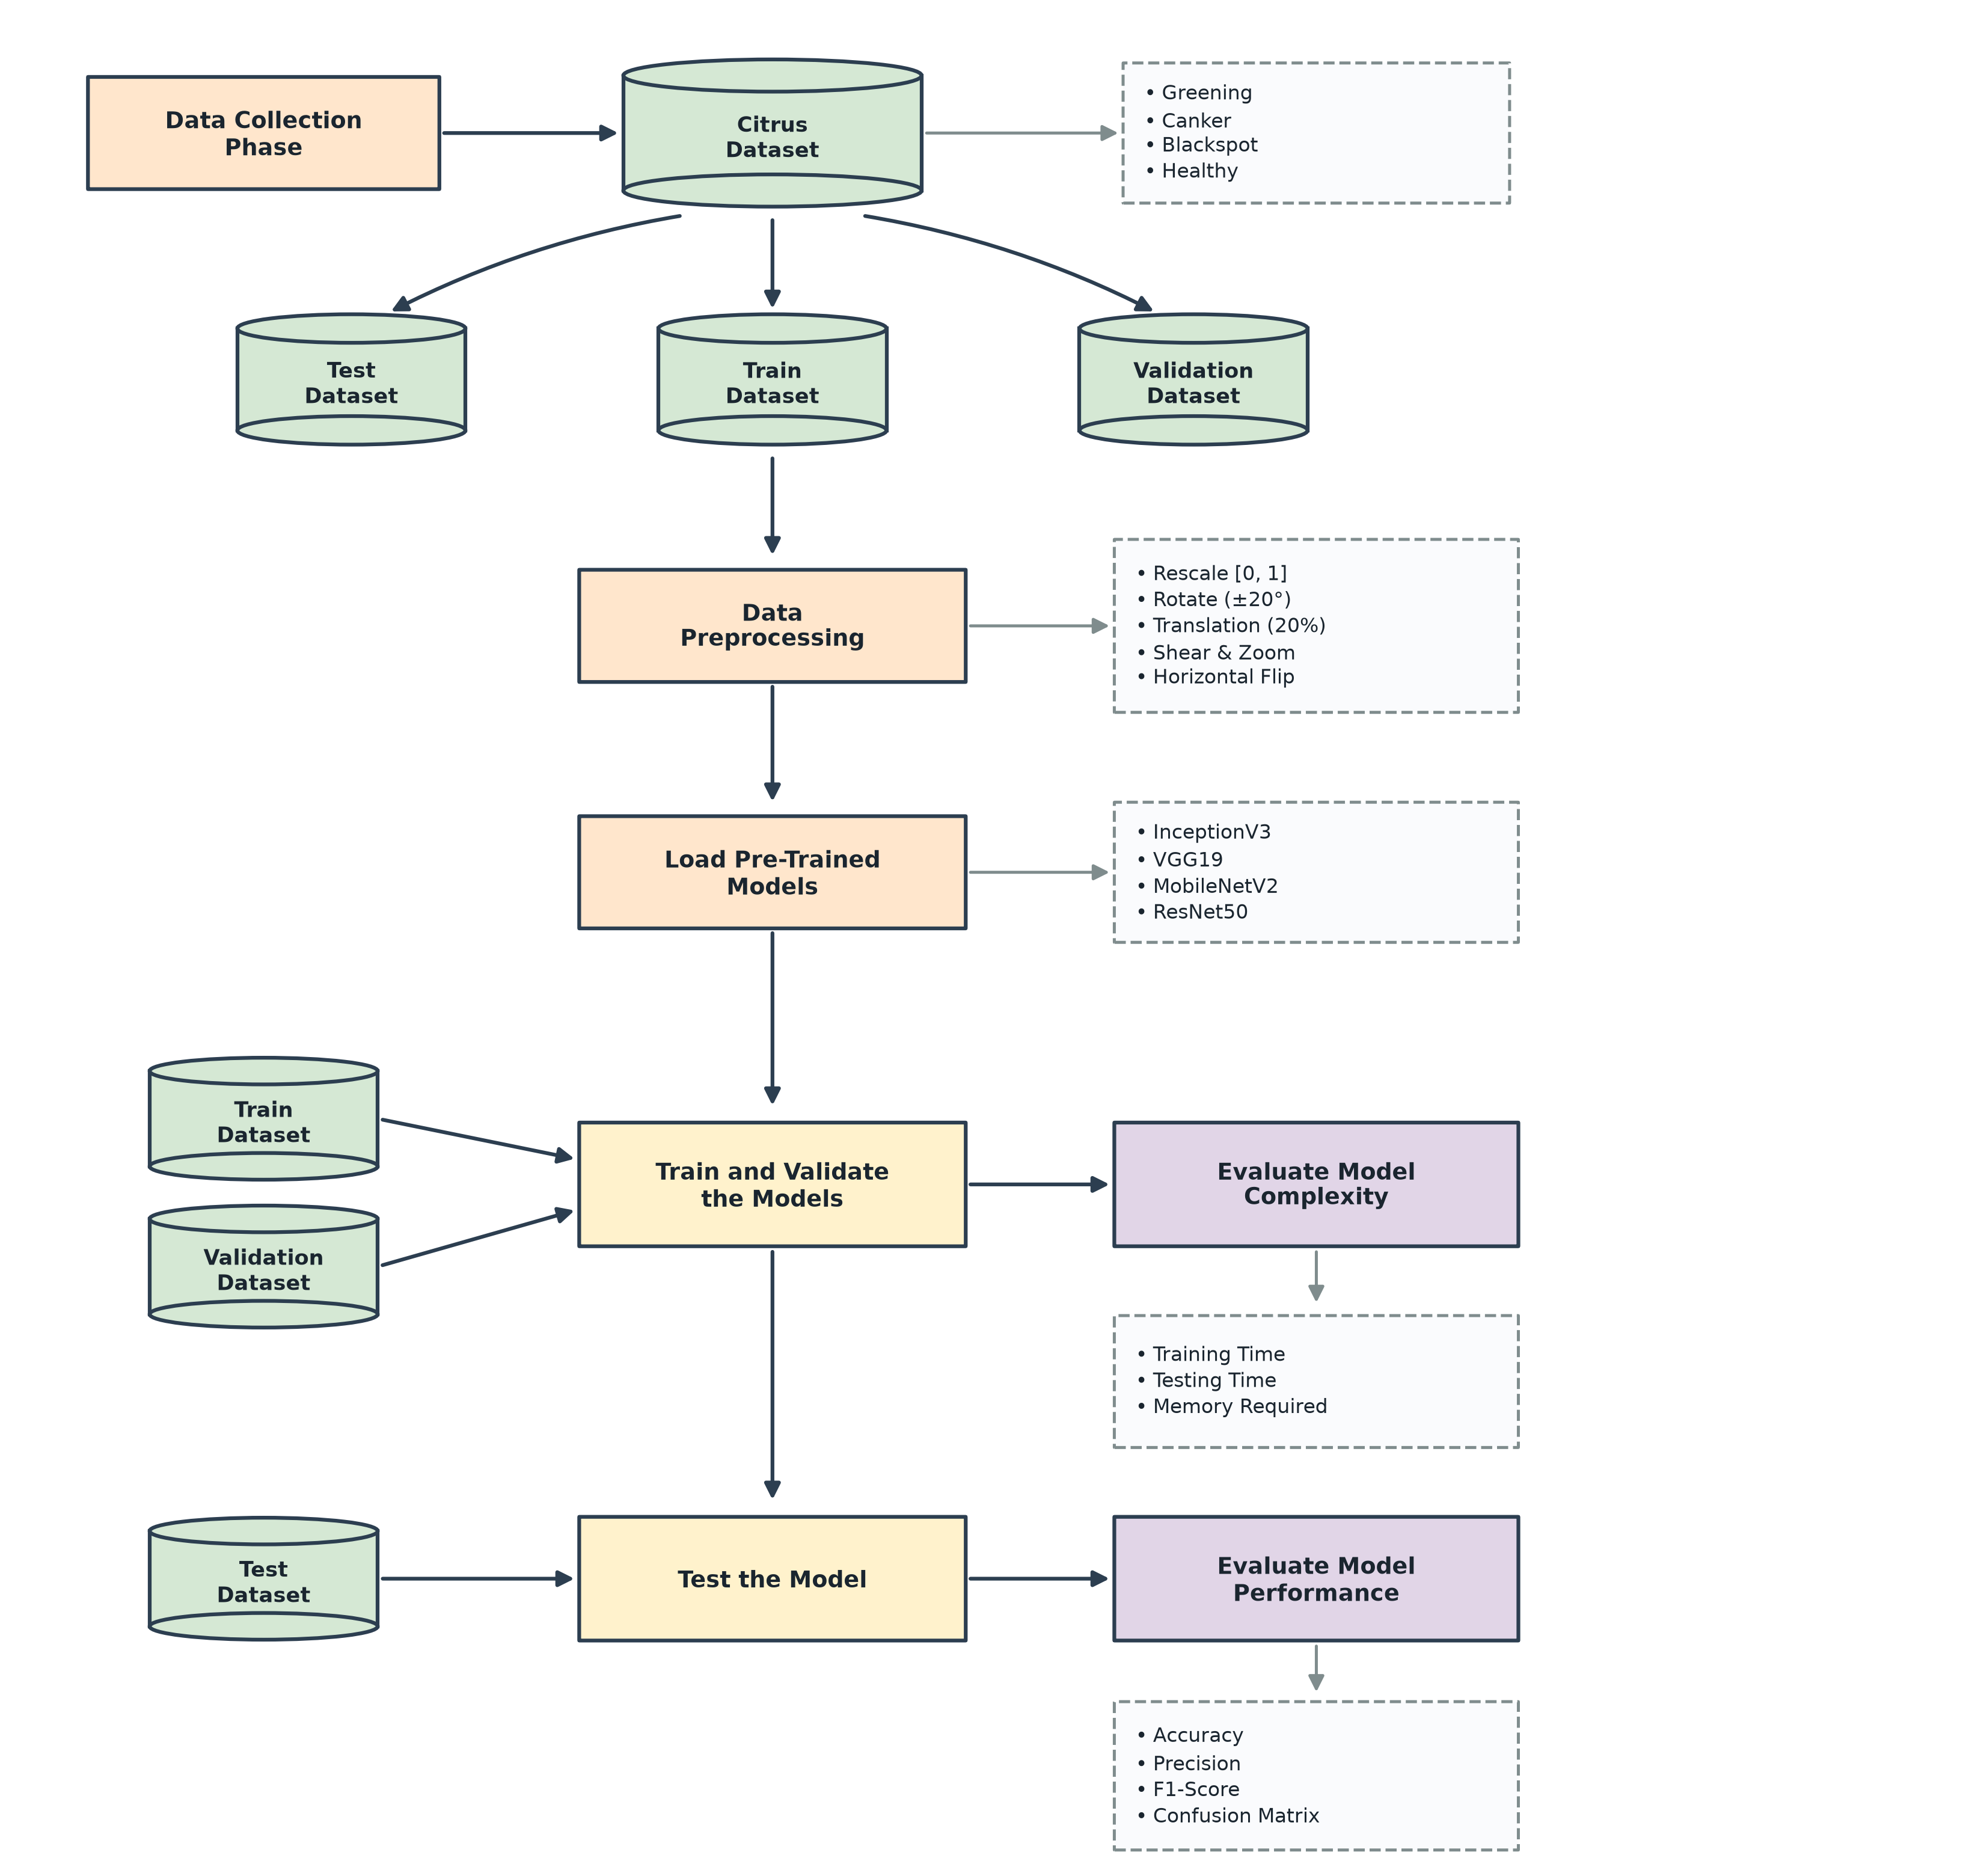
\includegraphics[width=0.88\columnwidth]{Untitled Diagram.png}}
    \caption{End-to-end methodological framework for citrus fruit disease classification.}
    \label{fig:research design}
\end{figure}

\subsection{Dataset Overview and Preparation}
The experimental dataset comprises 1,463 high-resolution RGB images gathered from PlantVillage and Kaggle repositories. The dataset covers four primary condition classes:
\begin{itemize}
    \item \textbf{Canker}: Bacterial lesions caused by \textit{Xanthomonas citri}.
    \item \textbf{Black Spot}: Fungal lesions caused by \textit{Phyllosticta citricarpa}.
    \item \textbf{Greening (HLB)}: Vector-transmitted bacterial disease.
    \item \textbf{Healthy}: Asymptomatic citrus fruit samples.
\end{itemize}

\subsubsection{Class Distribution and Partitioning}
Images are organized in class-specific directories, with metadata mapped to a structured DataFrame. Figure~\ref{fig:class} illustrates the sample distribution across all four classes, confirming a balanced representation: 358 healthy, 387 greening, 362 black spot, and 356 canker samples. Figure~\ref{fig:sample images} presents visual samples for each category.

\begin{figure}[t]
    \centerline{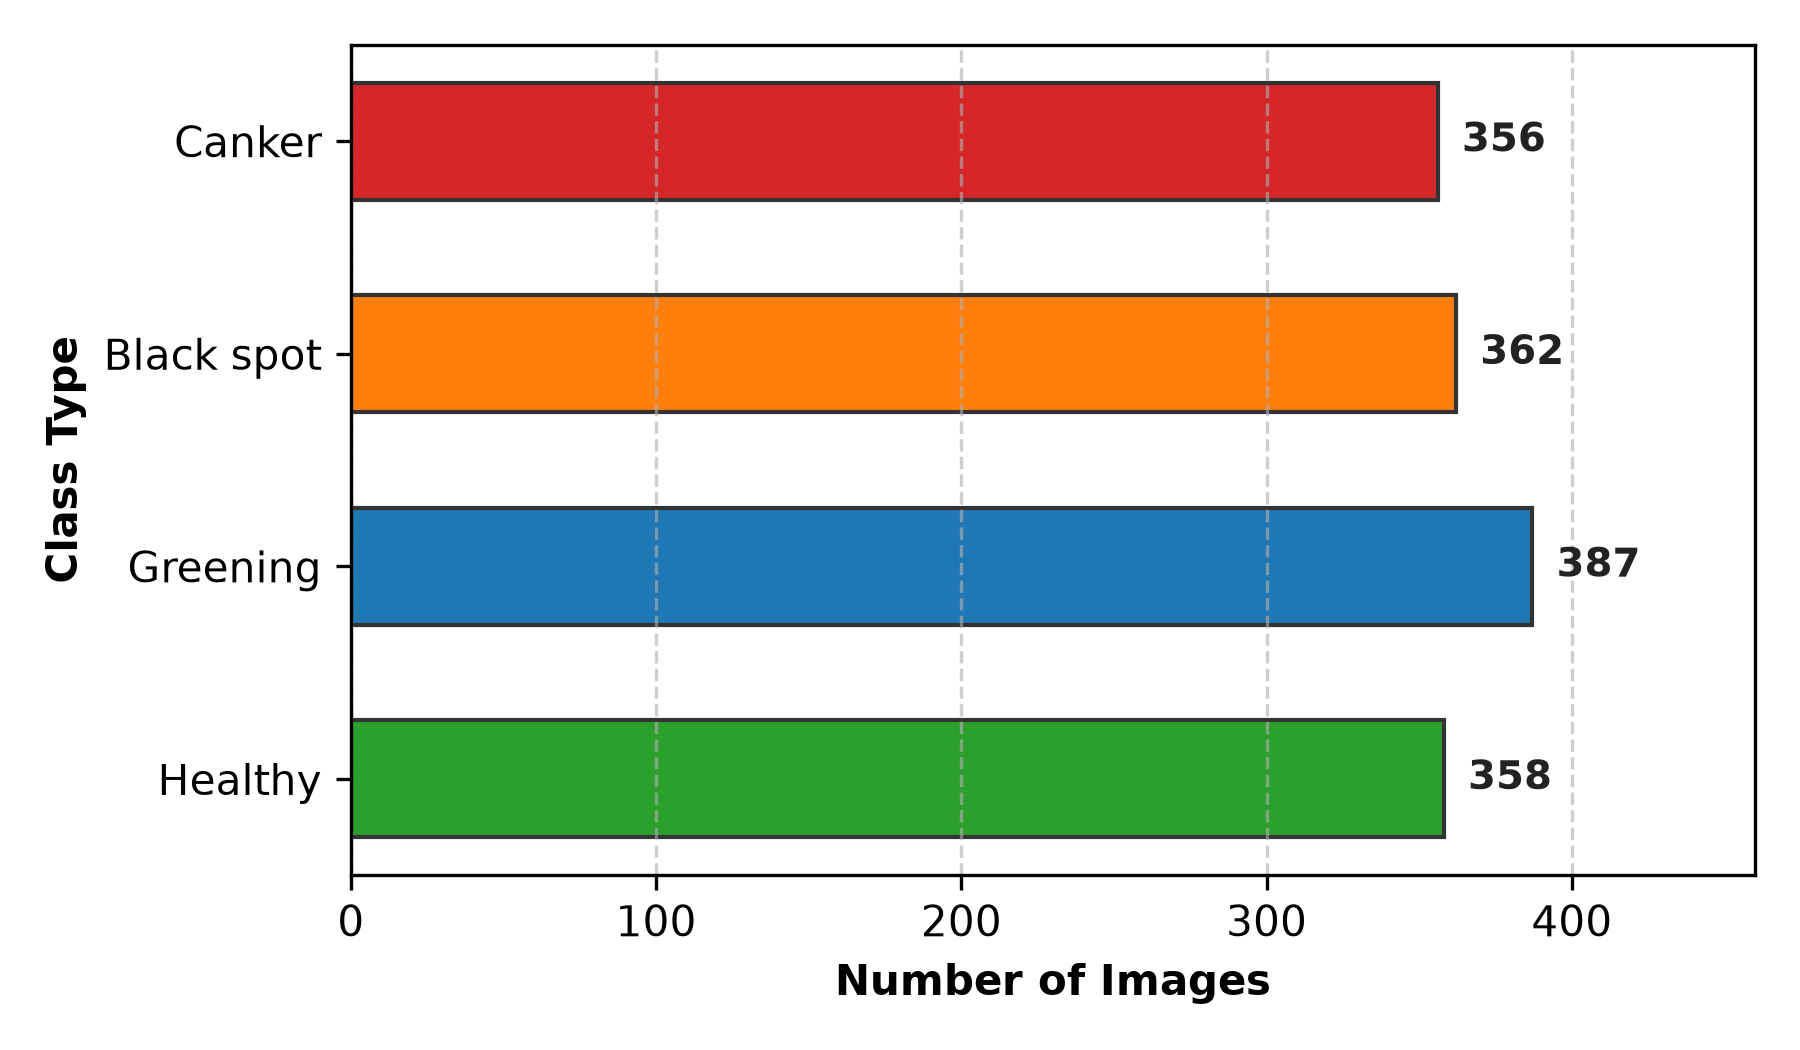
\includegraphics[width=0.88\columnwidth]{dataset visualization.png}}
    \caption{Distribution of image samples across the four citrus fruit classes.}
    \label{fig:class}
\end{figure}

\begin{figure}[t]
    \centerline{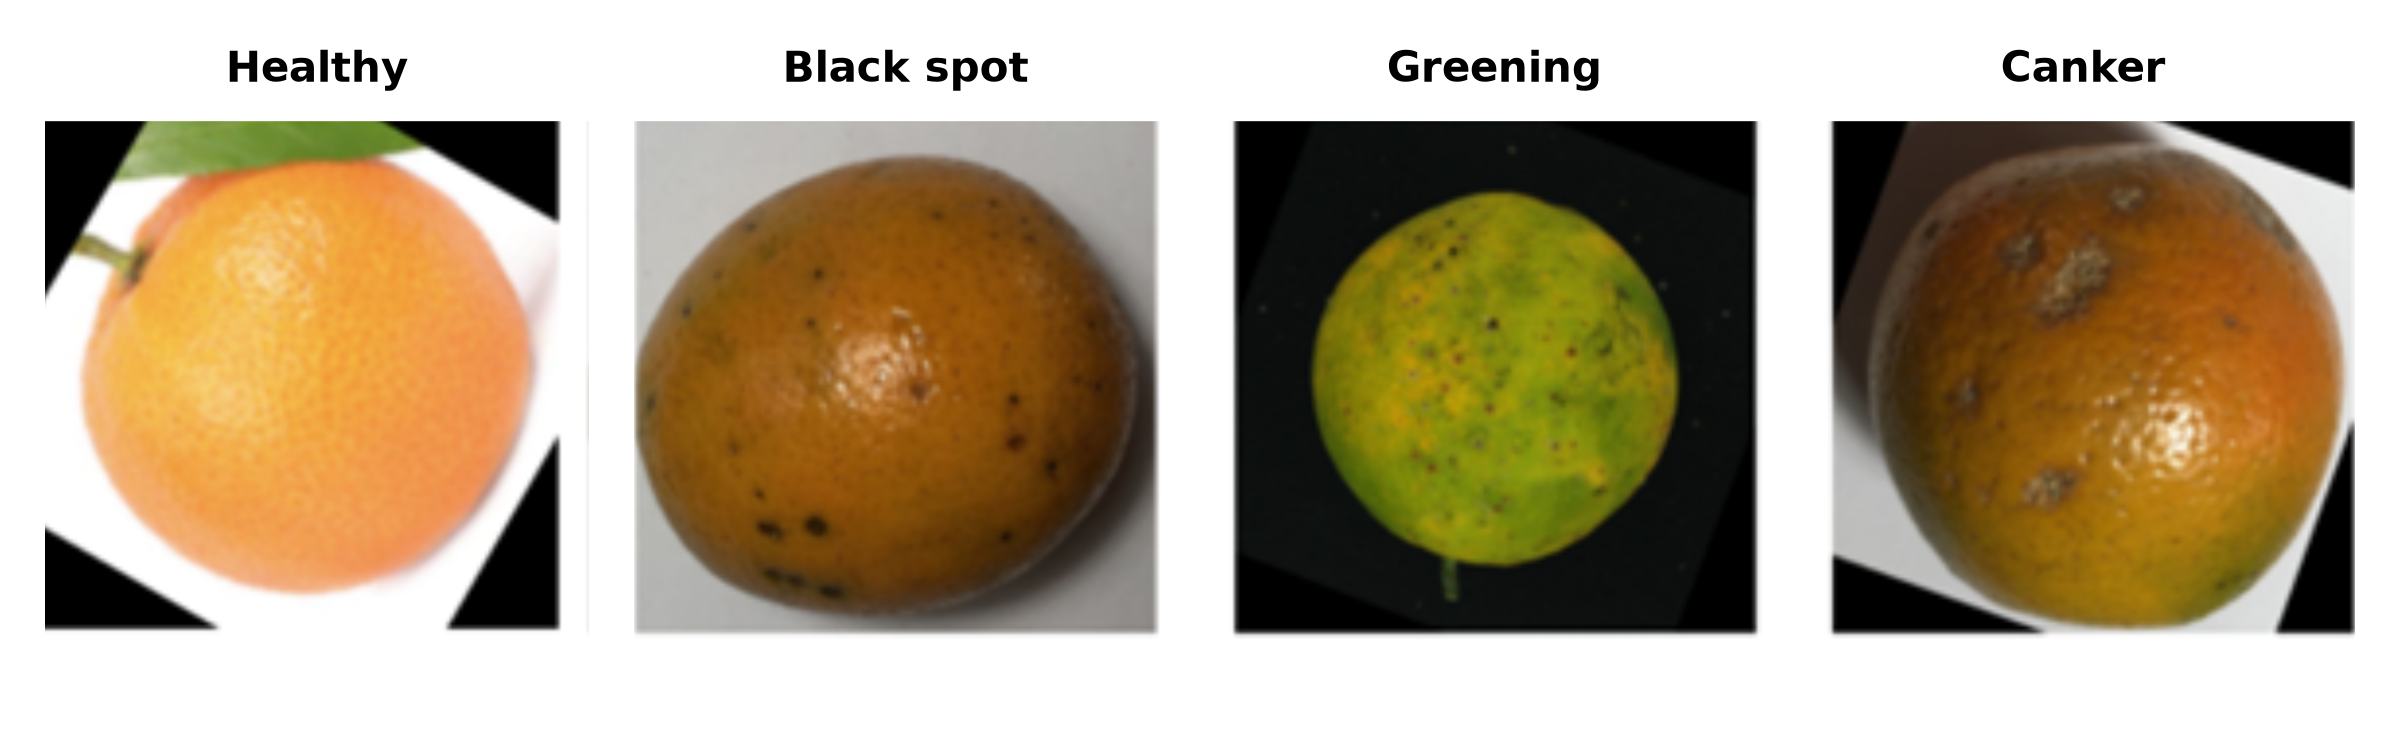
\includegraphics[width=0.88\columnwidth]{Sample images.png}}
    \caption{Representative sample images from the experimental citrus dataset.}
    \label{fig:sample images}
\end{figure}

The dataset is partitioned into 80\% for model training (1,170 images), 10\% for validation (146 images), and 10\% for unseen testing (147 images), as shown in Figure~\ref{fig:dataset split}. The test partition is held strictly separate to ensure unbiased evaluation.

\begin{figure}[t]
    \centerline{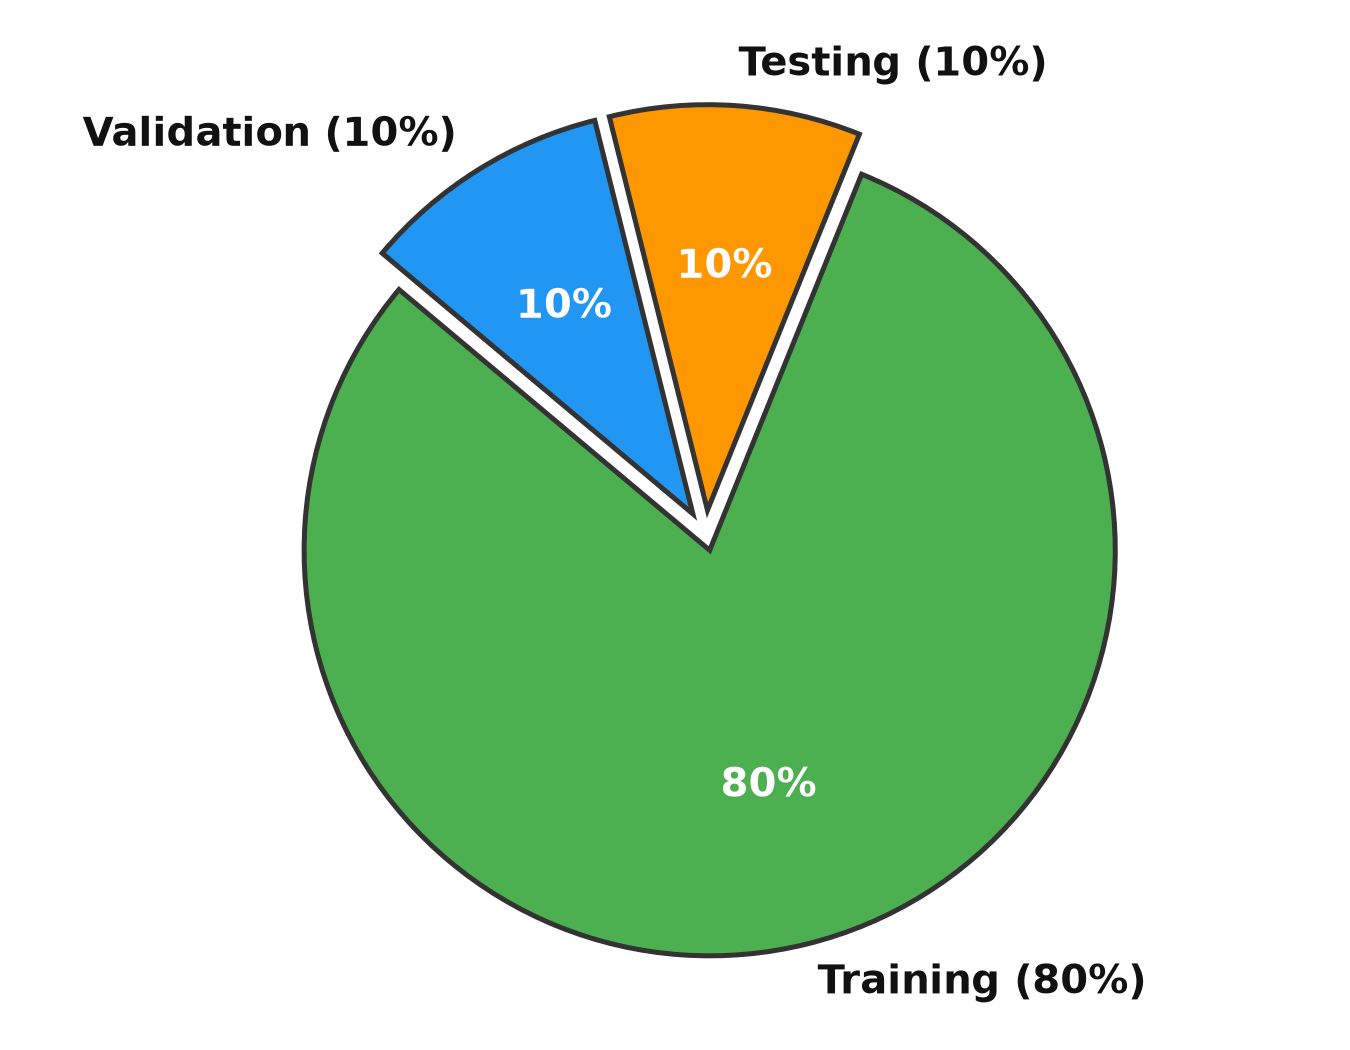
\includegraphics[width=0.72\columnwidth]{Dataset Spilt.png}}
    \caption{Dataset partitioning into training (80\%), validation (10\%), and test (10\%) subsets.}
    \label{fig:dataset split}
\end{figure}

\subsubsection{Data Pre-Processing and Augmentation}
To mitigate overfitting and enhance model robustness against environmental variations, data augmentation is applied to the training partition via real-time image generators:
\begin{itemize}
    \item Pixel intensity rescaling to the interval $[0, 1]$.
    \item Random rotation within $[-20^\circ, +20^\circ]$.
    \item Horizontal and vertical spatial translations up to 20\%.
    \item Random shear transformations.
    \item Random zoom variations up to 20\%.
    \item Random horizontal flipping.
\end{itemize}
All images are uniformly standardized to $224 \times 224 \times 3$ pixels with a mini-batch size of 32.

\subsection{Transfer Learning Framework}

Transfer learning leverages feature representations pre-trained on large-scale benchmark datasets (ImageNet) to accelerate convergence and enhance generalization on specialized domain-specific tasks \cite{p25,p24}. The transfer learning pipeline is illustrated in Figure~\ref{fig:pretrained}.

\begin{figure}[t]
    \centerline{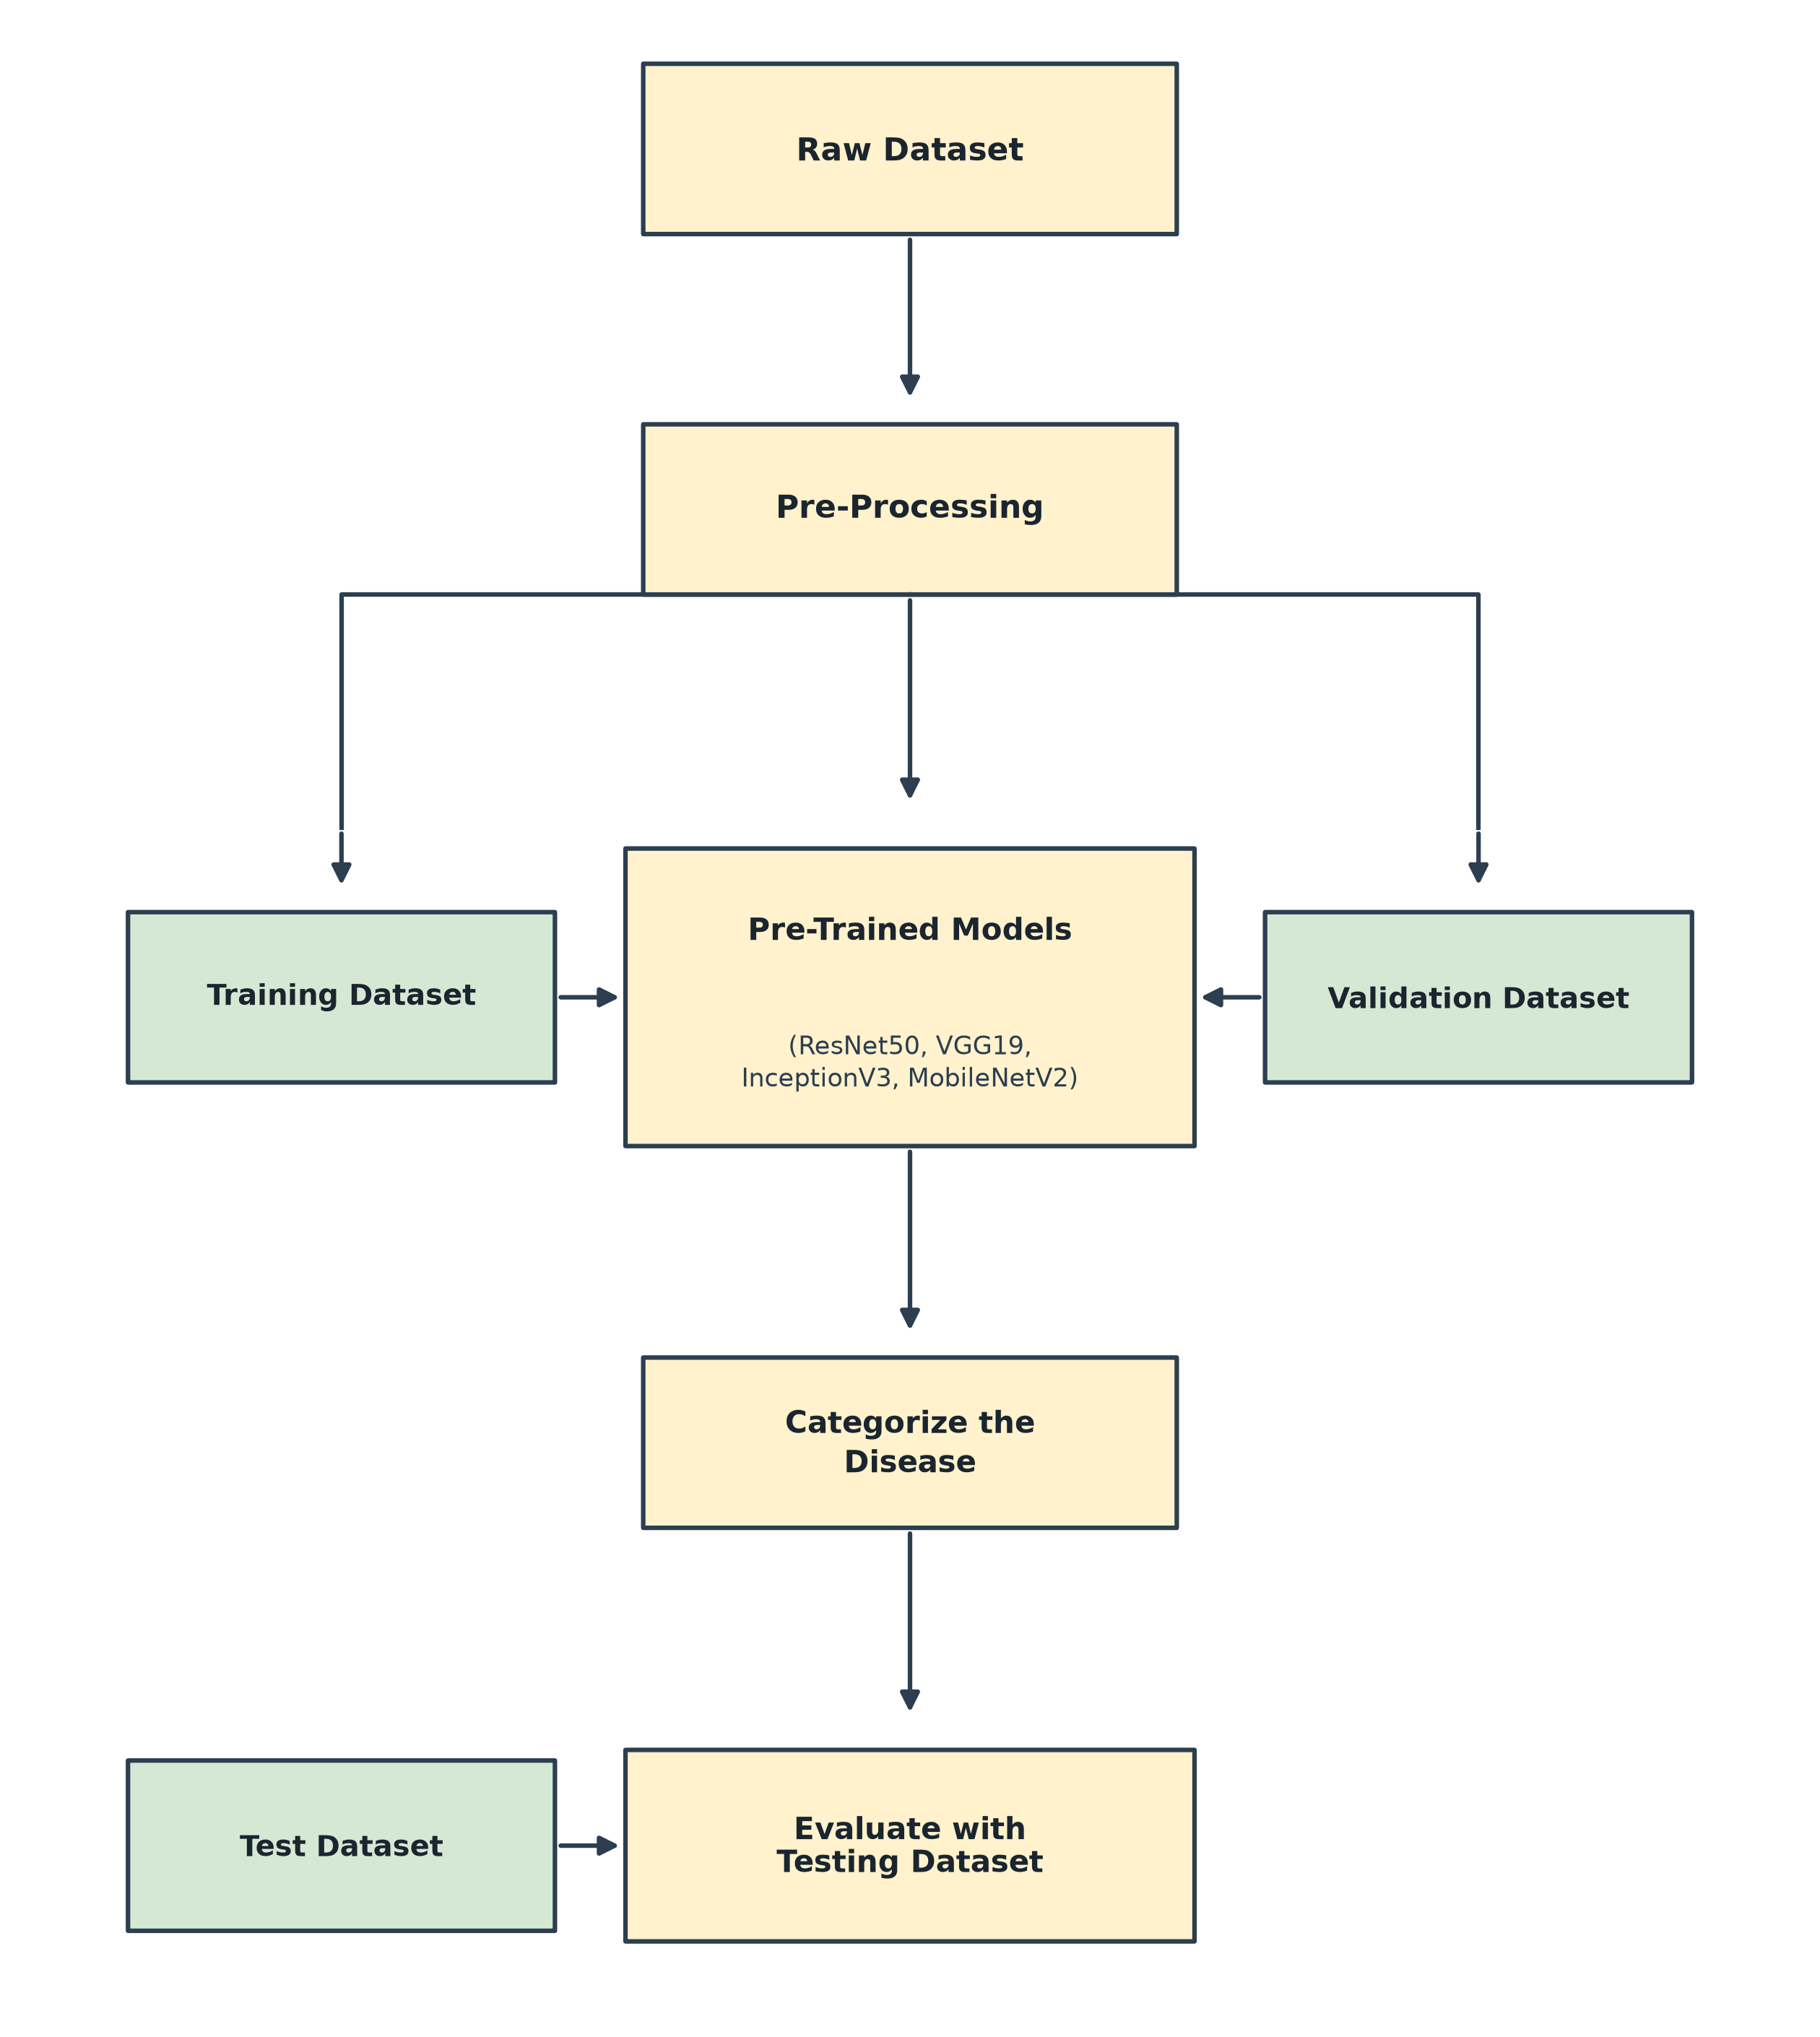
\includegraphics[width=0.72\columnwidth]{Pre-trained Process Diagram.png}}
    \caption{Flowchart of the transfer learning fine-tuning pipeline.}
    \label{fig:pretrained}
\end{figure}

Four distinct deep architectures were adapted:
\begin{itemize}
    \item \textbf{VGG19}: Consists of 19 layers characterized by uniform $3 \times 3$ convolutions \cite{p38,p39,p40}. The pre-trained convolutional base is frozen, followed by a 40\% Dropout layer \cite{p41,p42,p43}, a Flatten layer \cite{p44}, a Dense layer with 512 ReLU units, a 20\% Dropout layer, and a 4-unit Softmax output layer \cite{p45}. Table~\ref{tab:model_architecture} summarizes its layer configuration.

\begin{table}[htbp]
\tabcolsep4pt
\tbl{Layer Architecture and Parameter Details of Fine-Tuned VGG19}{
\begin{tabular}{|l|c|r|}
\hline
\textbf{Layer (Type)} & \textbf{Output Shape} & \textbf{Parameters} \\
\hline
VGG19 (Functional Base) & (None, 7, 7, 512) & 20,024,384 \\
dropout\_1 (Dropout 40\%) & (None, 7, 7, 512) & 0 \\
flatten (Flatten) & (None, 25088) & 0 \\
dense\_1 (Dense, ReLU) & (None, 512) & 12,845,056 \\
dropout\_2 (Dropout 20\%) & (None, 512) & 0 \\
dense\_2 (Dense, Softmax) & (None, 4) & 2,052 \\
\hline
\multicolumn{2}{|l|}{\textbf{Total Parameters:}} & 32,871,492 \\
\multicolumn{2}{|l|}{\textbf{Trainable Parameters:}} & 12,847,108 \\
\multicolumn{2}{|l|}{\textbf{Non-Trainable Parameters:}} & 20,024,384 \\
\hline
\end{tabular}}
\label{tab:model_architecture}
\end{table}

    \item \textbf{MobileNetV2}: Employs depthwise separable convolutions and inverted residual bottleneck blocks with linear bottlenecks \cite{p37}. The base feature extractor is frozen, followed by identical classification head regularization. Table~\ref{tab:mobilenetv2} provides the structural specifications.

\begin{table}[htbp]
\tabcolsep4pt
\tbl{Layer Architecture and Parameter Details of Fine-Tuned MobileNetV2}{
\begin{tabular}{|l|c|r|}
\hline
\textbf{Layer (Type)} & \textbf{Output Shape} & \textbf{Parameters} \\
\hline
MobileNetV2 (Base) & (None, 7, 7, 1280) & 2,257,984 \\
dropout\_1 (Dropout 40\%) & (None, 7, 7, 1280) & 0 \\
flatten (Flatten) & (None, 62720) & 0 \\
dense\_1 (Dense, ReLU) & (None, 512) & 32,085,760 \\
dropout\_2 (Dropout 20\%) & (None, 512) & 0 \\
dense\_2 (Dense, Softmax) & (None, 4) & 2,052 \\
\hline
\multicolumn{2}{|l|}{\textbf{Total Parameters:}} & 34,345,796 \\
\multicolumn{2}{|l|}{\textbf{Trainable Parameters:}} & 32,087,812 \\
\multicolumn{2}{|l|}{\textbf{Non-Trainable Parameters:}} & 2,257,984 \\
\hline
\end{tabular}}
\label{tab:mobilenetv2}
\end{table}

    \item \textbf{InceptionV3}: Implements multi-scale factorization with asymmetric convolutions for efficient representation learning. The custom head comprises a Flatten layer, Dense layer (512 units), Dropout regularization, and Softmax output. Table~\ref{tab:inceptionv3} presents the layer details.

\begin{table}[htbp]
\tabcolsep4pt
\tbl{Layer Architecture and Parameter Details of Fine-Tuned InceptionV3}{
\begin{tabular}{|l|c|r|}
\hline
\textbf{Layer (Type)} & \textbf{Output Shape} & \textbf{Parameters} \\
\hline
InceptionV3 (Base) & (None, 5, 5, 2048) & 21,802,784 \\
flatten (Flatten) & (None, 51200) & 0 \\
dense\_1 (Dense, ReLU) & (None, 512) & 26,214,912 \\
dropout\_2 (Dropout 20\%) & (None, 512) & 0 \\
dense\_2 (Dense, Softmax) & (None, 4) & 2,052 \\
\hline
\multicolumn{2}{|l|}{\textbf{Total Parameters:}} & 48,019,748 \\
\multicolumn{2}{|l|}{\textbf{Trainable Parameters:}} & 26,216,964 \\
\multicolumn{2}{|l|}{\textbf{Non-Trainable Parameters:}} & 21,802,784 \\
\hline
\end{tabular}}
\label{tab:inceptionv3}
\end{table}

    \item \textbf{ResNet50}: Incorporates residual skip connections to facilitate gradient backpropagation in deep networks. The top layers are replaced with custom Dense and Dropout layers. Table~\ref{tab:resnet50} outlines the architectural parameters.

\begin{table}[htbp]
\tabcolsep4pt
\tbl{Layer Architecture and Parameter Details of Fine-Tuned ResNet50}{
\begin{tabular}{|l|c|r|}
\hline
\textbf{Layer (Type)} & \textbf{Output Shape} & \textbf{Parameters} \\
\hline
ResNet50 (Base) & (None, 5, 5, 2048) & 23,587,712 \\
flatten (Flatten) & (None, 100352) & 0 \\
dense\_1 (Dense, ReLU) & (None, 512) & 51,380,736 \\
dropout\_2 (Dropout 50\%) & (None, 512) & 0 \\
dense\_2 (Dense, Softmax) & (None, 4) & 2,052 \\
\hline
\multicolumn{2}{|l|}{\textbf{Total Parameters:}} & 74,970,500 \\
\multicolumn{2}{|l|}{\textbf{Trainable Parameters:}} & 51,382,788 \\
\multicolumn{2}{|l|}{\textbf{Non-Trainable Parameters:}} & 23,587,712 \\
\hline
\end{tabular}}
\label{tab:resnet50}
\end{table}

\end{itemize}

\subsubsection{Framework Implementation}
Model development was executed in TensorFlow and Keras. The system architecture, spanning model instantiation, distributed training, serialization, and edge export formats (TensorFlow Lite, TensorFlow Serving), is shown in Figure~\ref{fig:tensorflow}.

\begin{figure}[t]
    \centerline{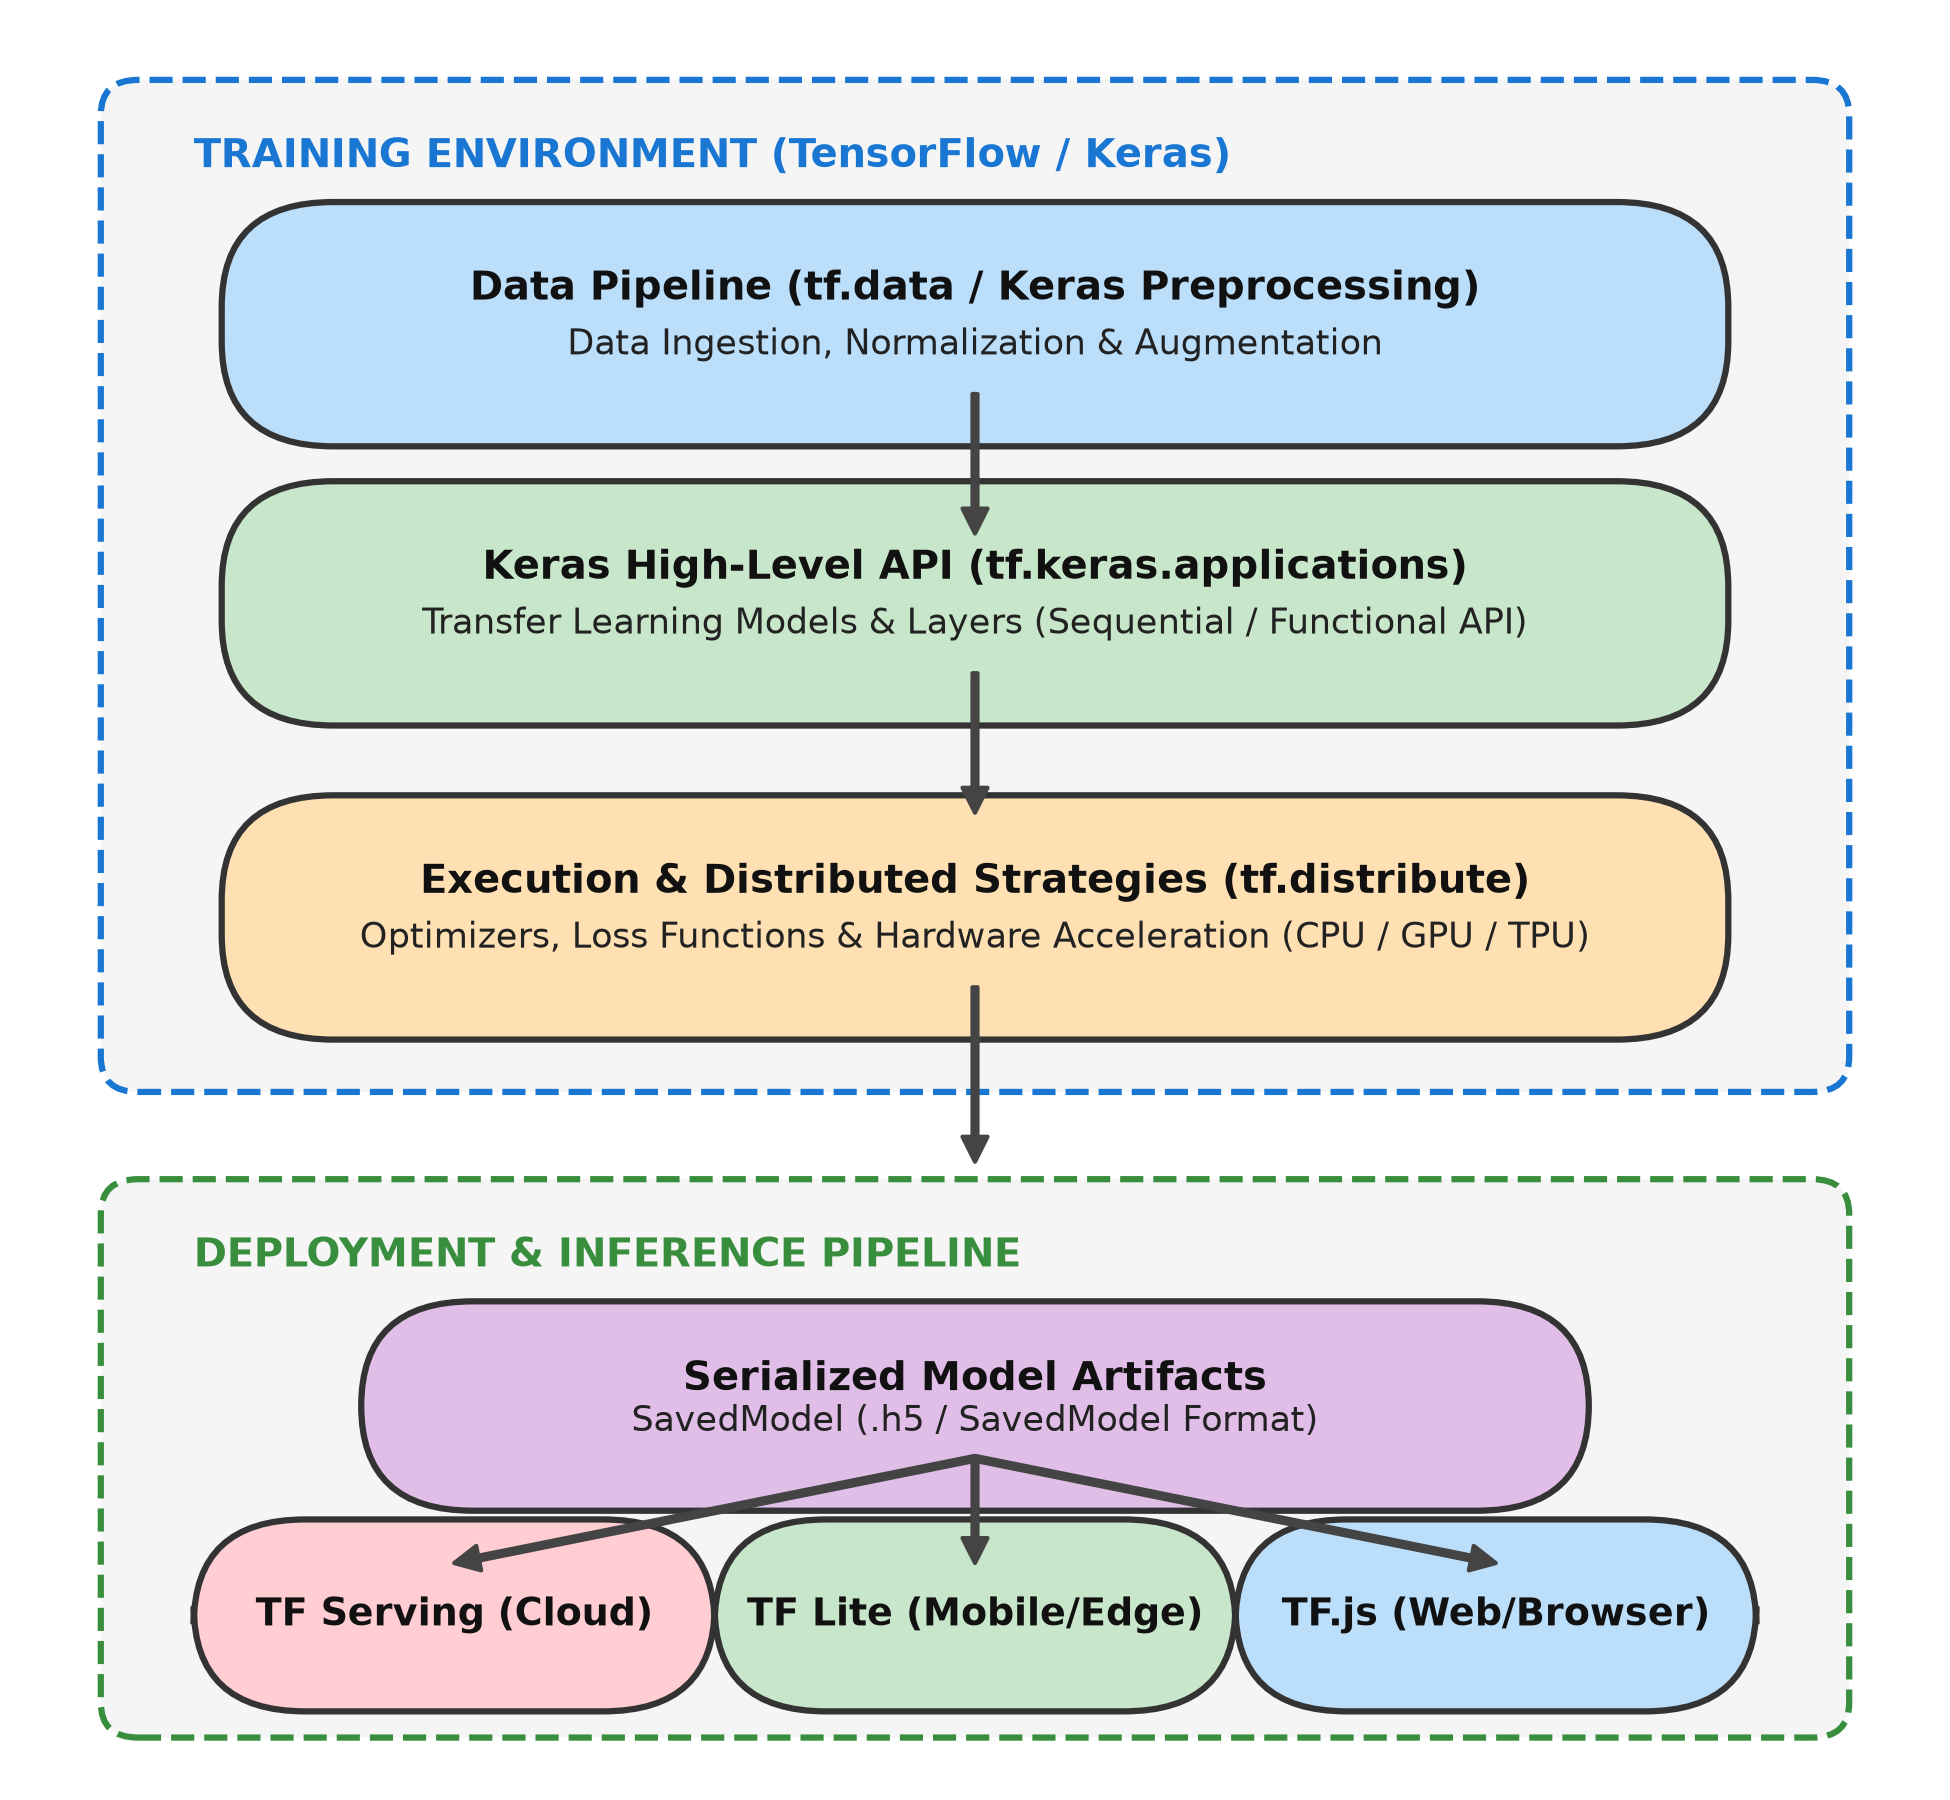
\includegraphics[width=0.88\columnwidth]{Tensorflow architecture.png}}
    \caption{Framework architecture covering training, serialization, and deployment pipelines.}
    \label{fig:tensorflow}
\end{figure}

\subsection{Optimization and Training Configuration}
All models were trained using the Adam optimizer with a learning rate of $\eta = 0.0001$. Categorical cross-entropy was employed as the objective loss function:
\begin{equation}
    \mathcal{L}_{CCE} = -\sum_{i=1}^{N} \sum_{c=1}^{C} y_{i,c} \log(\hat{y}_{i,c})
\end{equation}
where $N$ denotes batch size, $C=4$ is the number of disease classes, $y_{i,c}$ represents the ground truth one-hot label, and $\hat{y}_{i,c}$ denotes predicted class probability. Training proceeded for 50 epochs with checkpointing on validation loss.

\subsection{Evaluation Metrics}

\subsubsection{Diagnostic Performance Metrics}
Model classification performance is evaluated using standard statistical indicators:
\begin{equation}
    \text{Accuracy} = \frac{TP + TN}{TP + TN + FP + FN}
    \label{eq:accuracy}
\end{equation}
\begin{equation}
    \text{Precision} = \frac{TP}{TP + FP}
    \label{eq:precision}
\end{equation}
\begin{equation}
    \text{Recall} = \frac{TP}{TP + FN}
    \label{eq:recall}
\end{equation}
\begin{equation}
    F1\text{-Score} = \frac{2 \cdot \text{Precision} \cdot \text{Recall}}{\text{Precision} + \text{Recall}}
    \label{eq:f1score}
\end{equation}
where $TP$, $TN$, $FP$, and $FN$ correspond to True Positives, True Negatives, False Positives, and False Negatives, respectively.

\subsubsection{Computational Complexity Metrics}
Computational feasibility is quantified via total training duration (seconds), total test partition inference latency (seconds), total parameter count, and dynamic memory consumption (MB).

\section{Result and Discussion}
\label{sec:result_and_discussion}

This section presents empirical findings comparing diagnostic accuracy and computational efficiency across the evaluated architectures.

\subsection{Diagnostic Performance Evaluation}

Table~\ref{tab:performance_metrics} summarizes precision, recall, and F1-score across the four models. MobileNetV2 demonstrated the highest overall classification capability, securing 98.56\% precision, 98.54\% recall, and a 98.54\% F1-score. InceptionV3 closely followed with 97.21\% precision, 97.30\% recall, and a 97.19\% F1-score. Conversely, ResNet50 exhibited substantial performance degradation on the fine-tuning task, registering an F1-score of 58.21\%.

\begin{table}[htbp]
\tabcolsep4pt
\tbl{Performance Comparison Across Fine-Tuned Models on the Unseen Test Set}{
\begin{tabular}{|l|c|c|c|c|}
\hline
\textbf{Model Name} & \textbf{MobileNetV2} & \textbf{InceptionV3} & \textbf{ResNet50} & \textbf{VGG19} \\
\hline
Precision (\%) & 98.56 & 97.21 & 66.66 & 84.82 \\
Recall (\%) & 98.54 & 97.30 & 62.02 & 81.31 \\
F1-Score (\%) & 98.54 & 97.19 & 58.21 & 81.17 \\
\hline
\end{tabular}}
\label{tab:performance_metrics}
\end{table}

\subsubsection{Accuracy and Loss Trajectory Analysis}
Table~\ref{tab:evaluation_accuracy_loss} details train, validation, and test accuracies alongside corresponding loss values. MobileNetV2 achieved 97.29\% test accuracy with the lowest test loss (5.29\%). InceptionV3 attained 96.59\% test accuracy (7.44\% loss), while VGG19 reached 88.44\% test accuracy (37.76\% loss). ResNet50 recorded a test accuracy of 67.34\% and a high test loss of 76.16\%, demonstrating sensitivity to transfer learning without extensive layer unfreezing.

\begin{table}[htbp]
\tabcolsep2.5pt
\tbl{Accuracy and Loss Metrics Across Training, Validation, and Test Phases}{
\begin{tabular}{|l|c|c|c|c|c|c|}
\hline
\textbf{Model} & \multicolumn{2}{c|}{\textbf{Training}} &
\multicolumn{2}{c|}{\textbf{Validation}} &
\multicolumn{2}{c|}{\textbf{Testing}} \\
\hline
& \textbf{Acc. (\%)} & \textbf{Loss (\%)} &
\textbf{Acc. (\%)} & \textbf{Loss (\%)} &
\textbf{Acc. (\%)} & \textbf{Loss (\%)} \\
\hline
MobileNetV2 & 95.80 & 10.97 & 94.55 & 12.80 & 97.29 & 5.29 \\
InceptionV3 & 95.89 & 10.60 & 97.95 & 6.72 & 96.59 & 7.44 \\
ResNet50   & 57.14 & 96.91 & 61.90 & 83.92 & 67.34 & 76.16 \\
VGG19      & 75.10 & 60.10 & 87.75 & 32.46 & 88.44 & 37.76 \\
\hline
\end{tabular}}
\label{tab:evaluation_accuracy_loss}
\end{table}

\subsubsection{Confusion Matrix Analysis}
Figure~\ref{fig:confusion matrix} depicts the multi-class confusion matrices for all four architectures on the 147 test samples. MobileNetV2 and InceptionV3 exhibited minimal misclassifications across all four classes, achieving perfect separation on greening and near-perfect classification on canker and healthy samples.

\begin{figure}[t]
    \centerline{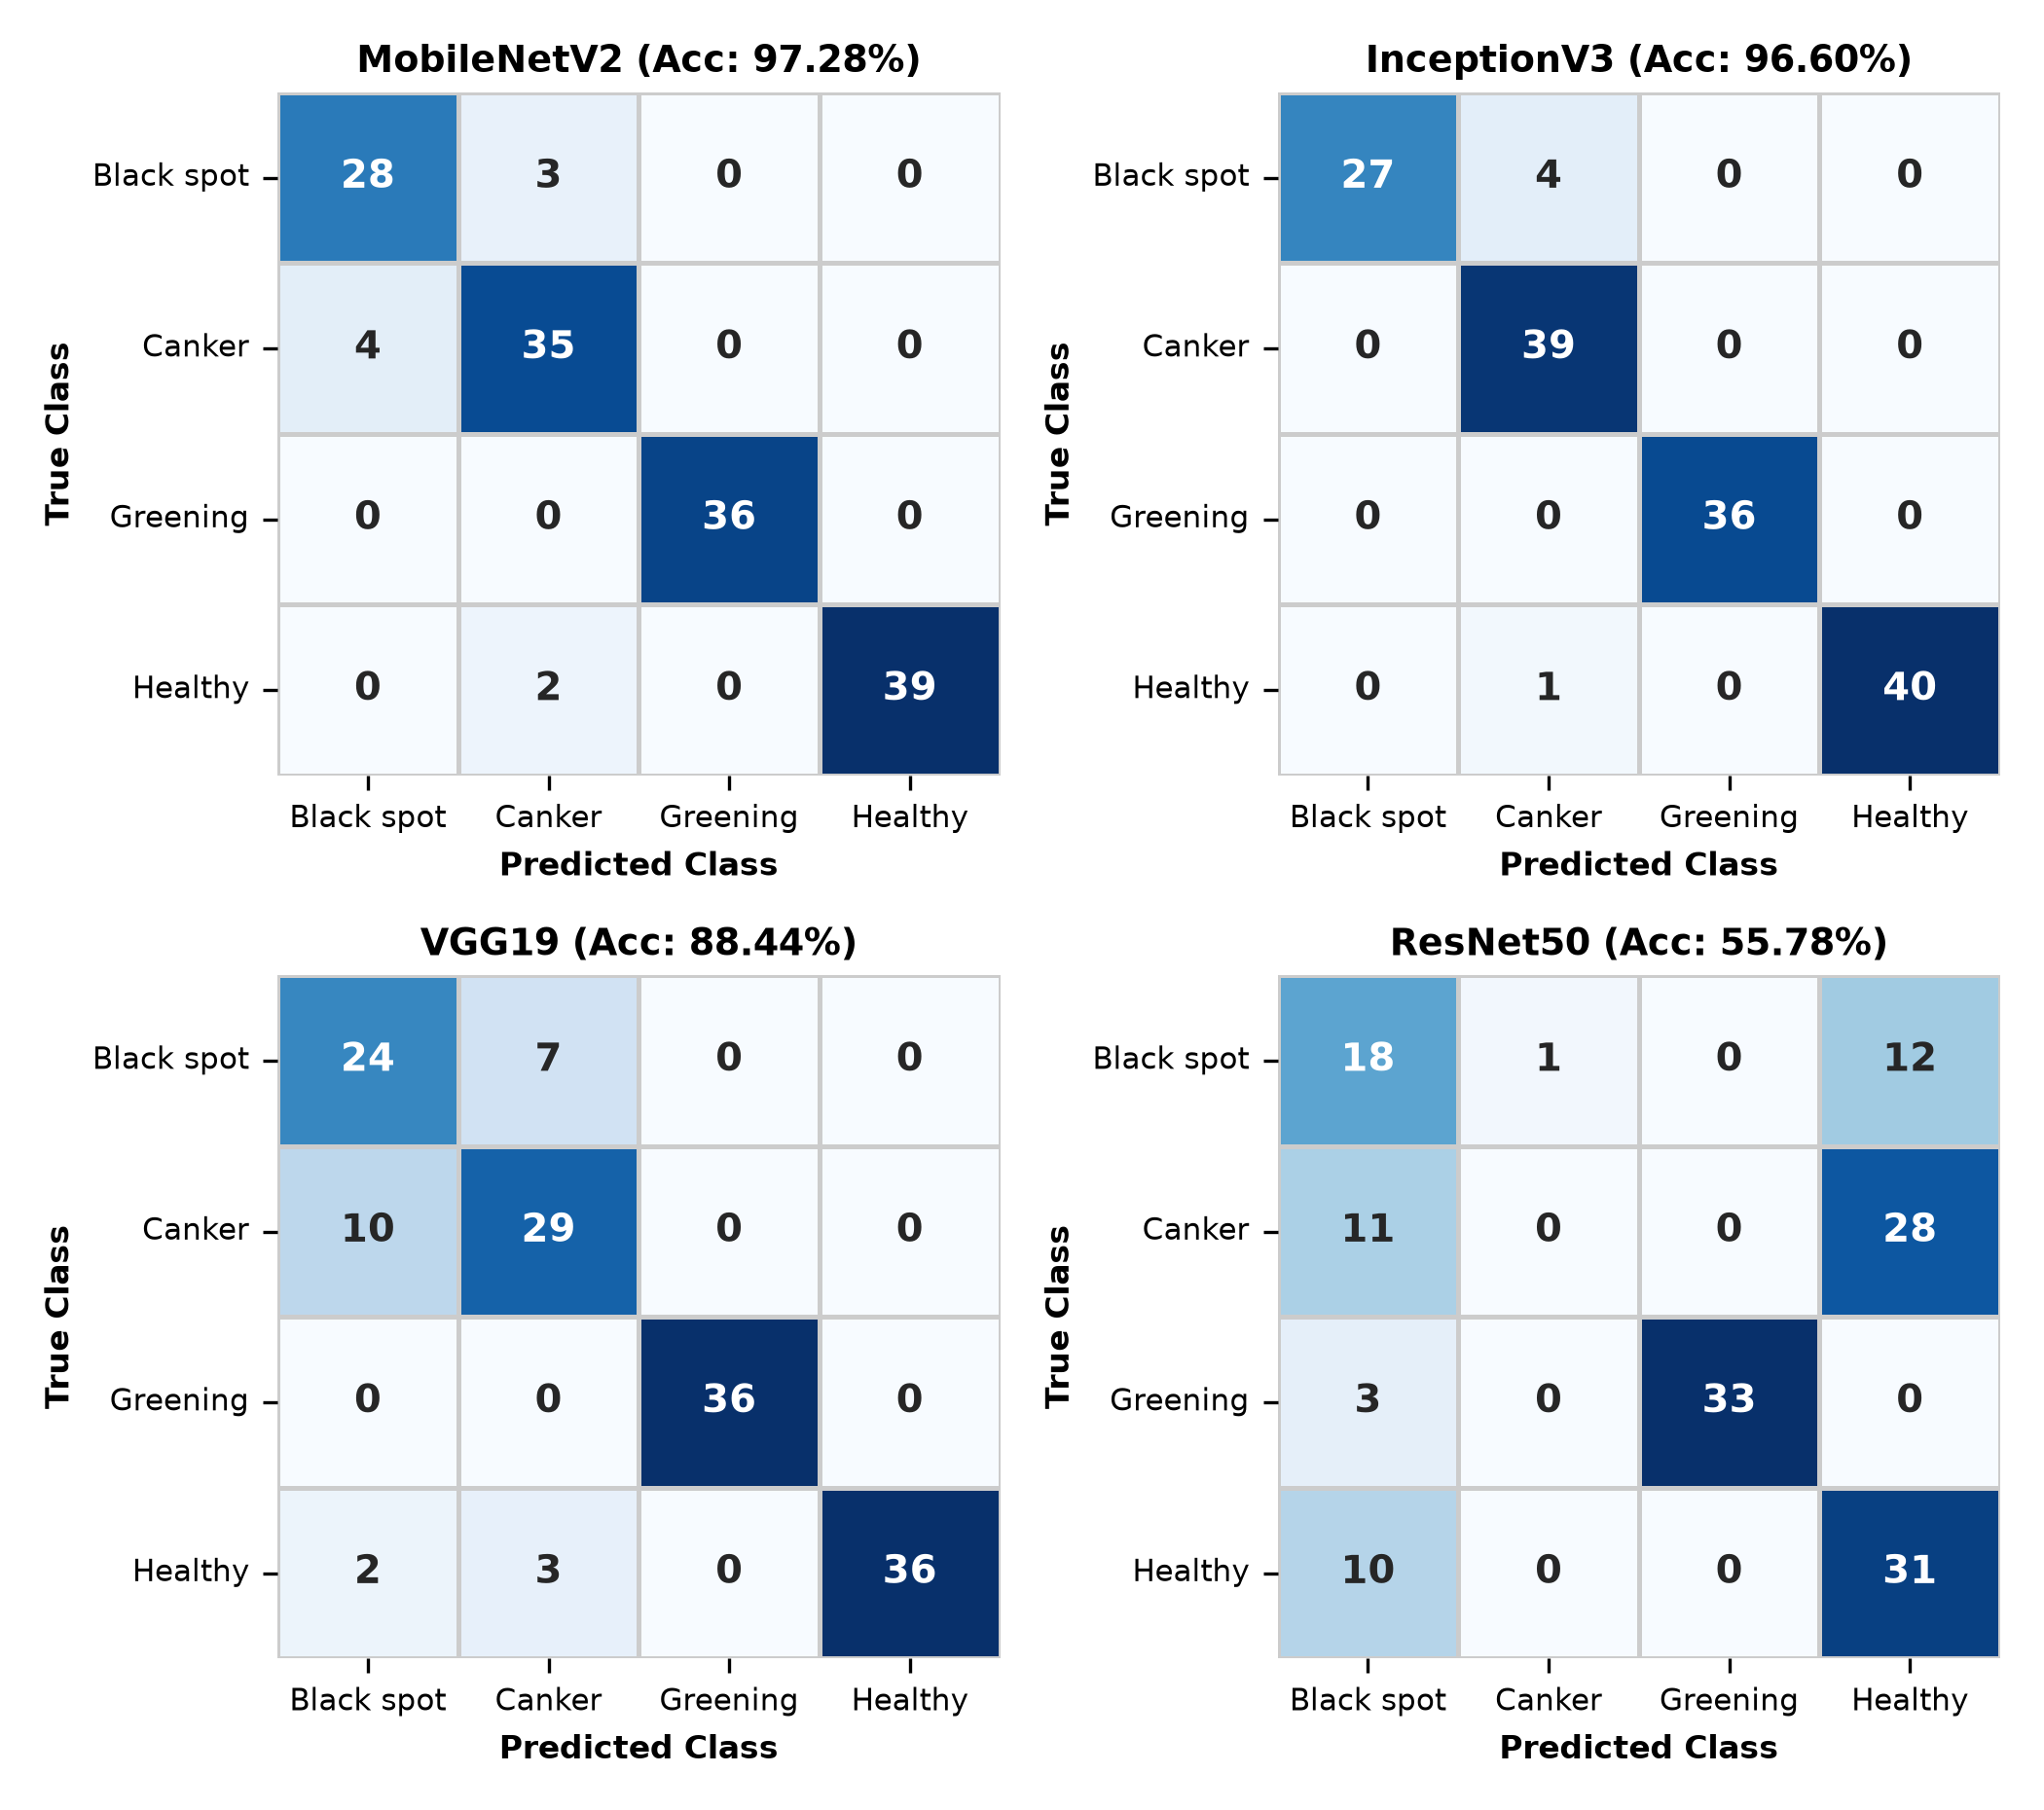
\includegraphics[width=0.88\columnwidth]{Confusion Matrix of all models.png}}
    \caption{Multi-class confusion matrices across all four fine-tuned CNN architectures on the test partition.}
    \label{fig:confusion matrix}
\end{figure}

\subsection{Computational Complexity Analysis}

In agricultural edge deployments, processing efficiency is as vital as diagnostic accuracy. Table~\ref{tab:complexity_metrics} compares training duration, inference latency, and memory requirements across models.

\begin{table}[htbp]
\tabcolsep4pt
\tbl{Quantitative Computational Complexity Metrics Across Models}{
\begin{tabular}{|l|c|c|c|c|}
\hline
\textbf{Metric} & \textbf{MobileNetV2} & \textbf{InceptionV3} &
\textbf{ResNet50} & \textbf{VGG19} \\
\hline
Training Time (s) & 406.29 & 717.00 & 1040.00 & 3360.14 \\
Inference Latency (s) & 83.67 & 85.73 & 84.11 & 80.34 \\
Memory Footprint (MB) & 9.82 & 22.81 & 34.28 & 118.59 \\
\hline
\end{tabular}}
\label{tab:complexity_metrics}
\end{table}

MobileNetV2 required the shortest training duration (406.29~s) and the lowest memory footprint (9.82~MB), representing an 88\% reduction in training duration and a 91.7\% reduction in memory compared to VGG19 (3360.14~s, 118.59~MB). Inference latencies remained comparable across all models ($\approx 80$--$85$~s for the 147 test samples). Figure~\ref{fig:performance metrics} graphically illustrates the performance metrics.

\begin{figure}[t]
    \centerline{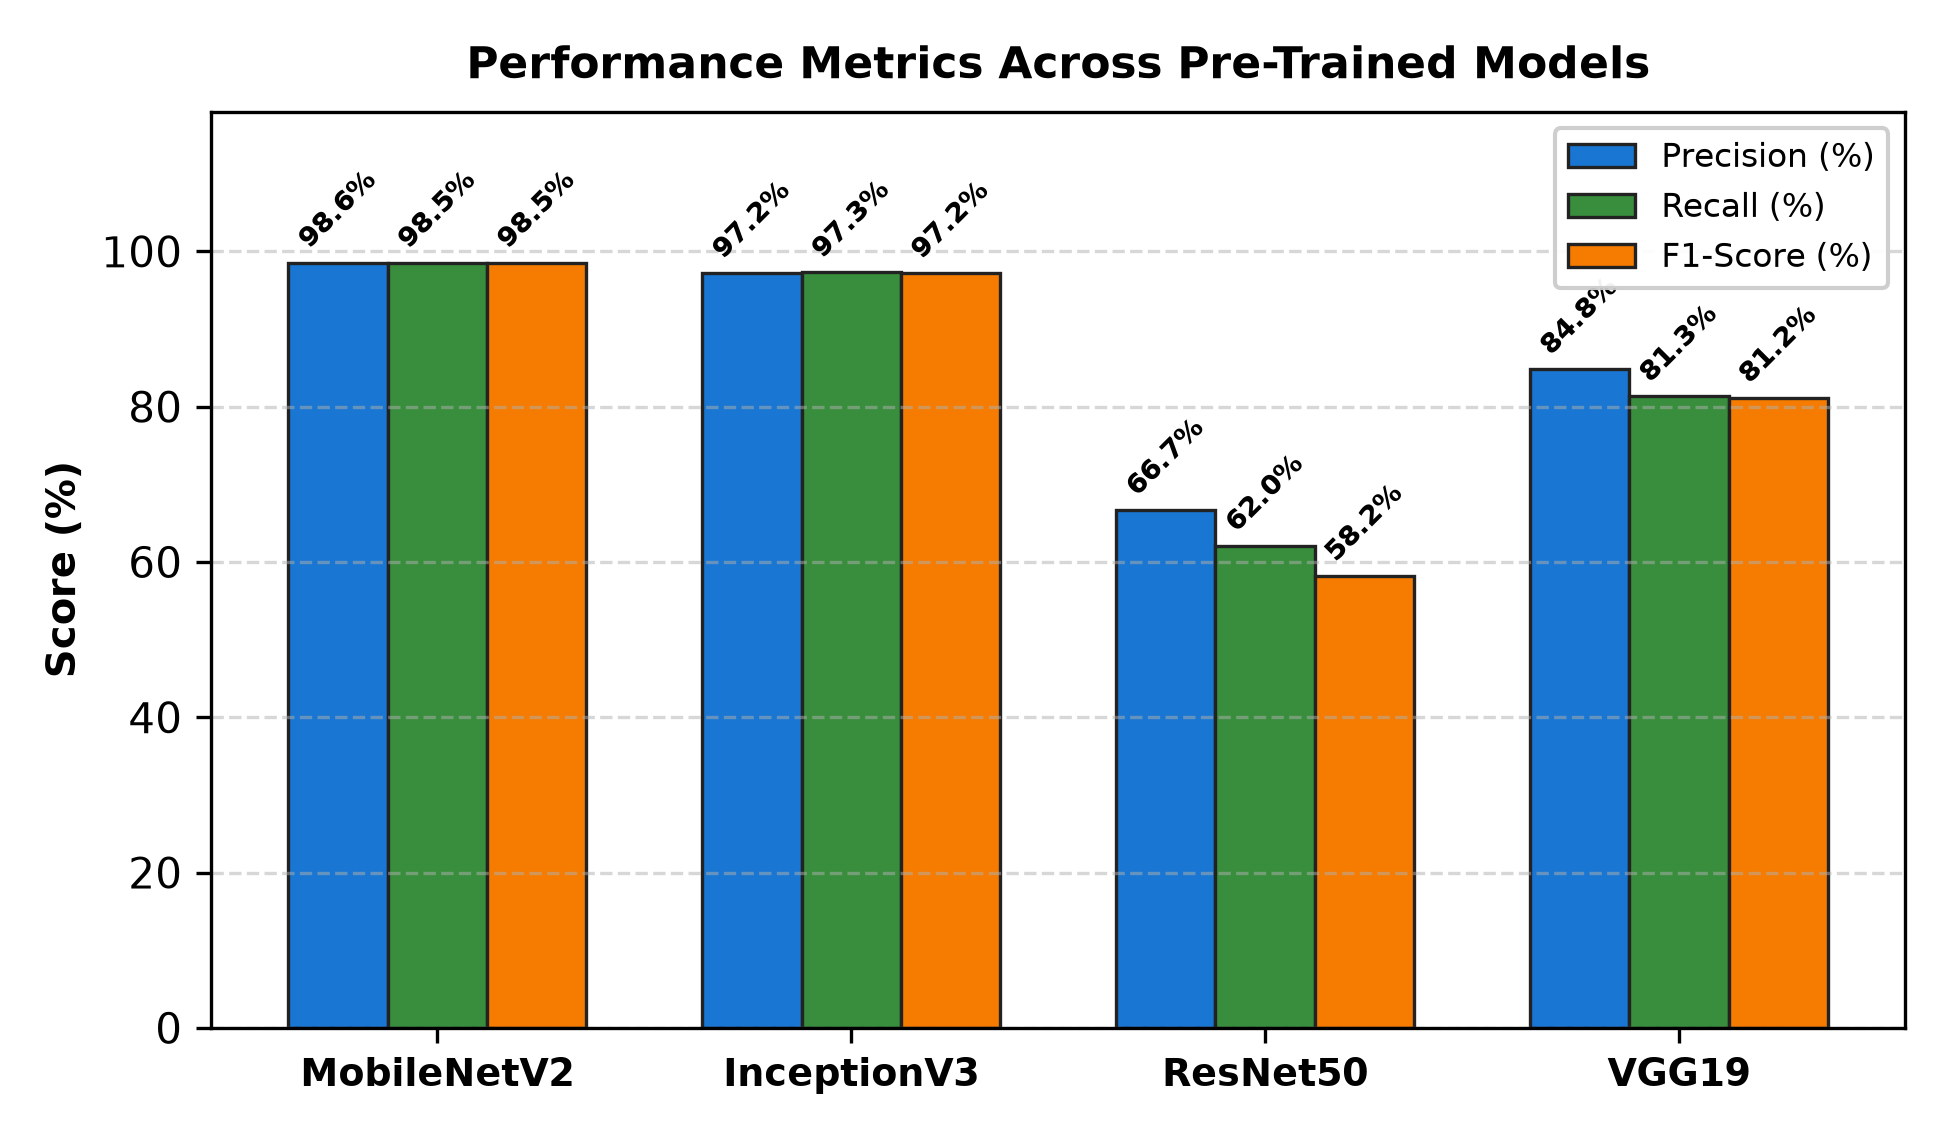
\includegraphics[width=0.88\columnwidth]{Performance metrics.png}}
    \caption{Comparative diagnostic metrics across the four pre-trained architectures.}
    \label{fig:performance metrics}
\end{figure}

\subsection{Comparative Discussion and Deployment Feasibility}

The empirical evaluation reveals that MobileNetV2 provides the optimal balance of diagnostic accuracy and computational frugality. Its inverted residual structure enables robust feature extraction without excessive parameterization. While InceptionV3 achieved comparable accuracy, its memory footprint (22.81~MB) and training overhead are higher. ResNet50 demonstrated poor feature adaptation under fixed-base fine-tuning, and VGG19 proved prohibitively heavyweight for low-power edge deployment.

Consequently, MobileNetV2 is identified as the most suitable candidate for integration into mobile applications, drone-based aerial imaging, and embedded edge devices in real-time orchard monitoring.

\section{Conclusion}
\label{sec:conclusion}

This research presented a comprehensive performance and computational complexity assessment of transfer learning architectures for citrus fruit disease classification. Evaluating MobileNetV2, InceptionV3, ResNet50, and VGG19 on a four-class dataset established MobileNetV2 as the superior model, achieving 96.77\% accuracy, 98.54\% F1-score, 406.29~s training time, and a 9.82~MB memory footprint. The results provide empirical evidence supporting the adoption of lightweight convolutional networks for scalable precision agriculture.

\subsection{Limitations}
The primary limitation of this study lies in the dataset scale (1,463 images) and single-source acquisition conditions. Field conditions frequently feature variable illumination, occlusion, and multi-disease co-occurrences that warrant expanded experimental datasets.

\subsection{Future Scope}
Future research directions include:
\begin{itemize}
    \item Integrating bio-inspired metaheuristic optimizers (e.g., Grey Wolf Optimizer, Particle Swarm Optimization) for automated hyperparameter tuning.
    \item Developing hybrid convolutional-transformer architectures.
    \item Incorporating Explainable AI (XAI) frameworks such as Grad-CAM to visualize pathological regions and foster user trust among agricultural practitioners.
\end{itemize}

\bibliographystyle{ijcaArticle}
\bibliography{References}

\end{document}
